\documentclass[a4paper,12pt]{article}

\usepackage[T2A]{fontenc}
\usepackage[utf8]{inputenc}
\usepackage[english,russian]{babel}
\usepackage{amsmath}
\usepackage{pgfplots}
\usepackage{geometry}
\usepackage{graphicx}
\usepackage[section,above,below]{placeins}
\usepackage{afterpage,placeins}
\usepackage{booktabs}
\usepackage{listings}
\usepackage{color}

\usepackage{algorithm}
\usepackage[noend]{algpseudocode}

\DeclareGraphicsExtensions{.png,.jpg}

\geometry{left=2cm}
\geometry{right=1.5cm}
\geometry{top=1cm}
\geometry{bottom=1.5cm}

\headheight = 1cm
\footskip = 0pt

\parskip = 4.25mm % расстояние между строками
\parindent=6.375mm % расстояние между абзацами
\floatname{algorithm}{Алгоритм} % переопределение имени в псевдокоде

\begin{document}
    \begin{titlepage}
        \begin{center}
            \large
            Государственное образовательное учреждение высшего профессионального образования\\
            “Московский государственный технический университет имени Н.Э.Баумана”
            \vspace{3cm}
            
            \textsc{Дисциплина: Анализ алгоритмов}
            \vspace{0.5cm}
                
            \textsc{Лабораторная работа №2}
            \vspace{3cm}
            
            {\LARGE Умножение матриц}
            \vspace{3cm}
            
            Студент группы ИУ7-54Б,\\   
            Котов Никита
            \vfill
            
            2019 г.            
            \end{center}
    \end{titlepage}
    
    \begin{center}
    	\tableofcontents
    \end{center}
	
	\setcounter{page}{2}
	\newpage
    \begin{center}
        \section*{Введение}
        \addcontentsline{toc}{section}{Введение}
    \end{center}
        \label{sec:intro}
\quad Матрица — математический объект, записываемый в виде прямоугольной таблицы элементов кольца или поля (например, целых или комплексных чисел), которая представляет собой совокупность строк и столбцов, на пересечении которых находятся её элементы. Количество строк и столбцов матрицы задают размер матрицы. Хотя исторически рассматривались, например, треугольные матрицы, в настоящее время говорят исключительно о матрицах прямоугольной формы, так как они являются наиболее удобными и общими.

Впервые матрицы упоминались ещё в древнем Китае, называясь тогда «волшебным квадратом». Основным применением матриц было решение линейных уравнений\cite{litlink1}. Так же, волшебные квадраты были известны чуть позднее у арабских математиков, примерно тогда появился принцип сложения матриц. После развития теории определителей в конце 17-го века, Габриэль Крамер начал разрабатывать свою теорию в 18-ом столетии и опубликовал «правило Крамера» в 1751 году. Примерно в этом же промежутке времени появился «метод Гаусса». Теория матриц начала своё существование в середине XIX века в работах Уильяма Гамильтона и Артура Кэли. Фундаментальные результаты в теории матриц принадлежат Вейерштрассу, Жордану, Фробениусу. Термин «матрица» ввел Джеймс Сильвестр в 1850 г\cite{litlink2}.

Матрицы широко применяются в математике для компактной записи систем линейных алгебраических или дифференциальных уравнений. В этом случае, количество строк матрицы соответствует числу уравнений, а количество столбцов — количеству неизвестных. В результате решение систем линейных уравнений сводится к операциям над матрицами.

Одной из основных операций над матрицами является умножение. Именно ему посвящена данная лабораторная работа. 
		
В рамках выполнения работы необходимо решить следующие задачи:   
		\begin{itemize}
		    \item рассмотреть стандартный алгоритм умножения матриц и алгоритм Винограда;
			\item реализовать каждый из этих алгоритмов, внеся в последний, как минимум 3 оптимизации;
			\item рассчитать их трудоемкость;
			\item сравнить временные характеристики реализованных алгоритмов экспериментально; 		
			\item на основании проделанной работы сделать выводы.
		\end{itemize}
    \newpage

    \begin{center}
        \section{Аналитическая часть}
	        \subsection{Описание алгоритмов}
    \end{center}
\subsubsection{Стандартный алгоритм}

Пусть даны две прямоугольные матрицы:
$$A_{lm} = 
\begin{pmatrix}
	a_{11} & a_{12} & ... & a_{1m}\\
	a_{21} & a_{22} & ... & a_{2m}\\
	\vdots & \vdots & \ddots & \vdots\\
	a_{l1} & a_{l2} & ... & a_{lm}
\end{pmatrix},\quad  
B_{mn} = 
\begin{pmatrix}
	b_{11} & b_{12} & ... & b_{1n}\\
	b_{21} & b_{22} & ... & b_{2n}\\
	\vdots & \vdots & \ddots & \vdots\\
	b_{m1} & b_{m2} & ... & b_{mn}
\end{pmatrix}
$$
Тогда матрица С 
$$C_{ln} = 
\begin{pmatrix}
	c_{11} & c_{12} & ... & c_{1n}\\
	c_{21} & c_{22} & ... & c_{2n}\\
	\vdots & \vdots & \ddots & \vdots\\
	c_{l1} & c_{l2} & ... & c_{ln}
\end{pmatrix},
$$
где:
\begin{equation}
\label{eq:M}
c_{ij} = 
 \sum_{r=1}^{m} a_{ir}b_{rj} \quad (i = 1,2,...l; j = 1,2,...n)
\end{equation}
будет называться произведением матриц A и B.
Стандартный алгоритм реализует данную формулу.

\subsubsection{Алгоритм Винограда}
Рассматривая результат умножения двух матриц очевидно, что каждый элемент в нем представляет собой скалярное произведение соответствующих строки и столбца исходных матриц. Такое умножение допускает предварительную обработку, позволяющую часть работы выполнить заранее.

Рассмотрим два вектора V = (v1, v2, v3, v4) и W = (w1, w2, w3, w4). Их скалярное произведение равно: \begin{equation}V * W = v1w1 + v2w2 + v3w3 + v4w4
\end{equation}

Это равенство можно переписать в виде: \begin{equation}V * W = (v1 + w2)(v2 + w1) + (v3 + w4)(v4 + w3) - v1v2 - v3v4 - w1w2 - w3w4
\end{equation}

Несмотря на то, что второе выражение требует вычисления большего количества операций, чем стандартный алгоритм: вместо четырех умножений - шесть, а вместо трех сложений - десять, выражение в правой части последнего равенства допускает предварительную обработку: его части можно вычислить заранее и запомнить для каждой строки первой матрицы и для каждого столбца второй, то для каждого элемента будет необходимо выполнить лишь первые два умножения и последующие пять сложений, а также дополнительно два сложения. Из-за того, что операция сложения быстрее операции умножения, алгоритм должен работать быстрее стандартного.

\begin{center}
\subsection{Модель вычислений}
\end{center}


Для последующего вычисления трудоемкости необходимо ввести модель вычислений:
\begin{enumerate}
\item +, -, /, \%, ==, !=, <, >, <=, >=, [], ++, \-- -- имеют трудоемкость 1
\item трудоемкость оператора выбора
			\begin{algorithmic}
			\If{\text{условие}}
				\State A
			\Else
				\State B
			\EndIf
			\end{algorithmic}
 рассчитывается, как 
			\[ f_{if} = f_{\text{условия}} + 
			\begin{cases}
				f_A, & \text{если условие выполняется,}\\
				f_B, & \text{иначе.}
			\end{cases} \]
\item трудоемкость цикла рассчитывается, как $f_{for} = f_{\text{инициализации}} + f_{\text{сравнения}} + N(f_{\text{тела}} + f_{\text{инициализации}} + f_{\text{сравнения}})$
\item трудоемкость вызова метода равна 0
\item трудоемкость вызова функции равна 1
\end{enumerate}

    \newpage

    \begin{center}
        \section{Конструкторская часть}
        \subsection{Разработка алгоритмов}
        \subsubsection{Cтандартный алгоритм умножения матриц}
    \end{center}
	
	На рис.~\ref{ris:simple} представлена схема стандартного алгоритма умножения матриц
	 		\begin{figure}[H]
	 			\centering
	 			{
	 				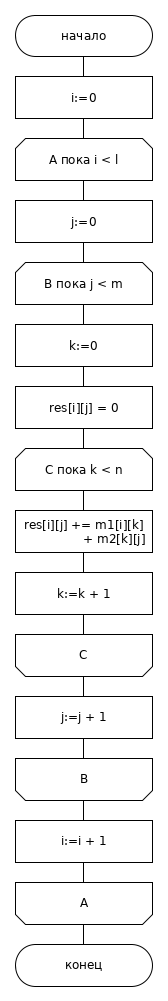
\includegraphics[scale=0.51]{simple_mult.png}
	 				\caption{\label{ris:simple}Стандартный алгоритм умножения матриц}	
	 			}
	 		\end{figure}
	
	Видно, что для стандартного алгоритма не существует лучшего и худшего случаев, как таковых.
    \newpage
    
    \afterpage{\FloatBarrier}
    \subsubsection{Алгоритм Винограда}
    
    На рис.~\ref{ris:vin1} и рис.~\ref{ris:vin2} приведена схема алгоритма Винограда
	 		\begin{figure}[H]
	 			\centering
	 			{
	 				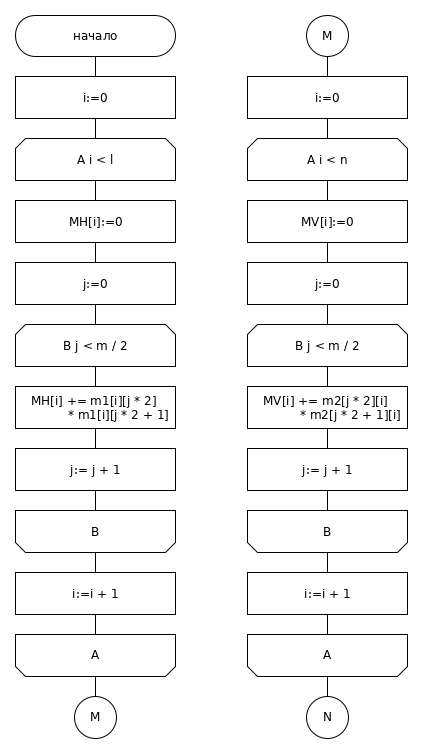
\includegraphics[scale=0.51]{vinograd1.png}
	 				\caption{\label{ris:vin1}Алгоритм Винограда}	
	 			}
	 		\end{figure}	
	 		\begin{figure}[H]
	 			\centering
	 			{
	 				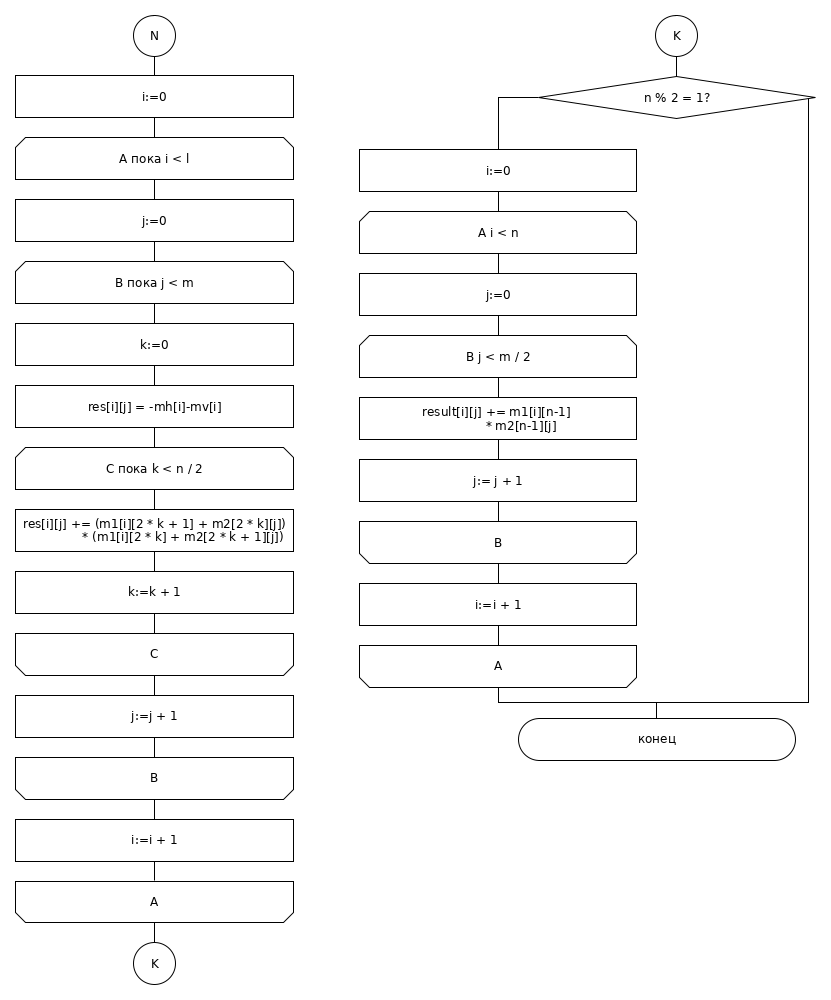
\includegraphics[scale=0.51]{vinograd2.png}
	 				\caption{\label{ris:vin2}Алгоритм Винограда}	
	 			}
	 		\end{figure}
	
	Видно, что для алгоритма Виноградова худшим случаем являются матрицы нечетного размера, а лучшим четного, т.к. отпадает необходимость в последнем цикле.\\
	В качестве оптимизаций можно:
	\begin{itemize}
	\item заранее считать в MH и MV отрицательные произведения
	\item заменить выражения вида $a = a + ...$ на $a += ...$
	\item в циклах по k сделать шаг 2, избавившись тем самым от двух операций умножения на каждую итерацию
	\end{itemize}
    \newpage	
    
    \begin{center}
    	\subsection{Выводы по конструкторскому разделу}    
    \end{center}
   
    	\qquad Были разработаны схемы обоих алгоритмов умножения матриц. Оценены лучшие и худшие случаи их работы, выбраны методы оптимизации.
    	
    \newpage
    
    \begin{center}
     	\section{Технологическая часть}
        \subsection{Средства реализации}    
    \end{center}
    
		В качестве языка программирования был выбран C++, так как он предоставляет широкие возможности для эффективной реализации алгоритмов.
	\begin{center}
	\end{center}

    \begin{center}
        \subsection{Листинг кода}    
    \end{center}
				\lstset{
	        		language=C++,
	        		basicstyle=\ttfamily,
	        		keywordstyle=\color{blue}\ttfamily,
	        		stringstyle=\color{red}\ttfamily,
	        		commentstyle=\color{green}\ttfamily,
	        		morecomment=[l][\color{magenta}]{\#},
	        		columns=fullflexible,
	        	    tabsize=1, 
	        		breakatwhitespace=true
	        	}
        	
        		\begin{lstlisting}[frame=single,caption=Стандартный алгоритм умножения матриц, breaklines]
matrix_d common_multiplication(matrix_d &m1, matrix_d &m2) {
    auto l = m1.size();
    auto m = m2.size();
    auto n = m2[0].size();

    if (m1[0].size() != m) {
        throw std::exception();
    }

    auto result = init_matrix(l, n);

    for (size_t i = 0; i < l; i++) {
        for (size_t j = 0; j < n; j++) {
            for (int k = 0; k < m; k++) {
                result[i][j] += m1[i][k] * m2[k][j];
            }
        }
    }

    return result;
}
        		\end{lstlisting}        		
    
            	\begin{lstlisting}[frame=single,caption=Алгоритм винограда, breaklines]
row_d bad_get_negative_row_products(matrix_d &matrix, size_t m, size_t n) {
    auto result = row_d(m, 0.);
    for (size_t i = 0; i < m; i++) {
        for (size_t j = 0; j <= n / 2; j++) {
            result[i] = result[i] + matrix[i][j * 2] * matrix[i][j * 2 + 1];
        }
    }

    return result;
}

row_d bad_get_negative_col_products(matrix_d &matrix, size_t m, size_t n) {
    auto result = row_d(m, 0.);
    for (size_t i = 0; i < m; i++) {
        for (size_t j = 0; j <= n / 2; j += 2) {
            result[i] = result[i] + matrix[2 * j][i] * matrix[2 * j + 1][i];
        }
    }

    return result;
}

matrix_d bad_vinograd_multiplication(matrix_d &m1, matrix_d &m2) {
    auto l = m1.size();
    auto m = m2.size();
    auto n = m2[0].size();

    if (m1[0].size() != m) {
        throw std::exception();
    }

    auto mh = bad_get_negative_row_products(m1, l, m);
    auto mv = bad_get_negative_col_products(m2, n, m);

    auto result = init_matrix(l, n);
    for (size_t i = 0; i < l; i++) {
        for (size_t j = 0; j < m; j++) {
            result[i][j] = -mh[i] - mv[j];
            for (size_t k = 0; k <= n / 2; k++) {
                result[i][j] = result[i][j] + (m1[i][2 * k + 1] + m2[2 * k][j]) * (m1[i][2 * k] + m2[2 * k + 1][j]);
            }
        }
    }

    if (n % 2 == 1) {
        for (size_t i = 0; i < l; i++) {
            for (size_t j = 0; j < m; j++) {
                result[i][j] = result[i][j] + m1[i][n - 1] * m2[n-1][j];
            }
        }
    }

    return result;
}
   				 \end{lstlisting}
    \newpage
            	\begin{lstlisting}[frame=single,caption=Алгоритм Винограда с оптимизациями, breaklines]
row_d get_negative_row_products(matrix_d &matrix, size_t m, size_t n) {
    auto result = row_d(m, 0.);
    for (size_t i = 0; i < m; i++) {
        for (size_t j = 0; j < n - 1; j += 2) {
            result[i] -= matrix[i][j] * matrix[i][j + 1];
        }
    }

    return result;
}

row_d get_negative_col_products(matrix_d &matrix, size_t m, size_t n) {
    auto result = row_d(m, 0.);
    for (size_t i = 0; i < m; i++) {
        for (size_t j = 0; j < n - 1; j += 2) {
            result[i] -= matrix[j][i] * matrix[j + 1][i];
        }
    }

    return result;
}

matrix_d vinograd_multiplication(matrix_d &m1, matrix_d &m2) {
    auto l = m1.size();
    auto m = m2.size();
    auto n = m2[0].size();

    if (m1[0].size() != m) {
        throw std::exception();
    }

    auto mh = get_negative_row_products(m1, l, m);
    auto mv = get_negative_col_products(m2, n, m);

    auto result = init_matrix(l, n);
    for (size_t i = 0; i < l; i++) {
        for (size_t j = 0; j < m; j++) {
            result[i][j] = mh[i] + mv[j];
            for (size_t k = 0; k < n - 1; k += 2) {
                result[i][j] += (m1[i][k + 1] + m2[k][j]) * (m1[i][k] + m2[k + 1][j]);
            }
        }
    }

    if (n % 2 == 1) {
        for (size_t i = 0; i < l; i++) {
            for (size_t j = 0; j < m; j++) {
                result[i][j] += m1[i][n - 1] * m2[n-1][j];
            }
        }
    }

    return result;
}
				\end{lstlisting}
    \newpage

	\begin{center}
		\subsection{Трудоемкость алгоритмов}
	\end{center}	    
    \textbf{Cтандартный алгоритм умножени матриц}
	$f = 2 + l(2 + 2 + n(2 + 2 + m(2 + 9)) = 11lmn + 4ln + 4l + 2$\\
	\textbf{Алгоритм Винограда}
	\begin{enumerate}
	\item $f_{row} = 2 + l(2 + 2 + 0.5n(2 + 10)) = 6ln + 4l + 2$
	\item $f_{col} = 2 + n(2 + 2 + 0.5m(2 + 10)) = 6mn + 4n + 2$
	\item $f_{matrix} = 2 + l(2 + 2 + m(2 + 2 + 7 + 0.5n(2 + 22)) = 12lmn + 11lm + 4l + 2$
	\item $f_{end} = \begin{cases}
	2, & \text{если матрица четная,}\\
	2 + 2 + l(2 + 2 + m(2 + 13)) = 15lm + 4l + 4, & \text{иначе.}
	\end{cases}$
	\end{enumerate}
	Итого, для худшего случая (нечетный размер матрицы) $f = f_{row} + f_{col} + f_{matrix} + f_{end} = 12lmn + 6ln + 6mn + 26lm + 12l + 4n + 10 \approx 12lmn$\\
	Для лучшего случая (четный размер матрицы: $f = f_{row} + f_{col} + f_{matrix} + f_{end} = 12lmn + 6ln + 6mn + 11lm + 8l + 4n + 8 \approx 12lmn$\\
	\textbf{Оптимизированный алгоритм Винограда}
	\begin{enumerate}
	\item $f_{row} = 2 + l(2 + 2 + 0.5n(2 + 8)) = 5ln - l + 2$
	\item $f_{col} = 2 + n(2 + 2 + 0.5m(2 + 8)) = 5mn - n + 2$
	\item $f_{matrix} = 2 + l(2 + 2 + m(2 + 2 + 5 + 0.5n(2 + 15)) = 8.5lmn + 9lm + 4l + 2$
	\item $f_{end} = \begin{cases}
	2, & \text{если матрица четная,}\\
	2 + 2 + l(2 + 2 + m(2 + 10)) = 12lm + 4l + 4, & \text{иначе.}
	\end{cases}$
	\end{enumerate}
	Итого, для худшего случая (нечетный размер матрицы) $f = f_{row} + f_{col} + f_{matrix} + f_{end} = 8.5lmn + 5ln + 5mn + 21lm + 7l - n + 10 \approx 8lmn$\\
	Для лучшего случая (четный размер матрицы): $f = f_{row} + f_{col} + f_{matrix} + f_{end} = 8.5lmn + 5ln + 5mn + 11lm + 3l - n + 8 \approx 8lmn$\\
	    
    
	\newpage    
    
    \begin{center}
		\subsection{Тестирование фунций}
	\end{center}		
	
	В таблице~\ref{tabular:test_rec} приведены тесты для функций, реализующих стандартный алгоритм умнодения матриц (СА), алгоритм Винограда (АВ) и оптимизированный алгоритм Винограда (АВ(О))
					\begin{table}[H]        		
       				\caption{\label{tabular:test_rec} Тестирование функций}
       				\begin{center}
        			\begin{tabular}{c@{\hspace{7mm}}c@{\hspace{7mm}}c@{\hspace{7mm}}c@{\hspace{7mm}}c@{\hspace{7mm}}c@{\hspace{7mm}}}        				
        				\hline
        				Матрица 1 & Матрица 2 &Ожидаемый результат &СА & АВ & АВ(О) \\ \hline
        				\vspace{4mm}
        				$\begin{pmatrix}
							1 & 2 & 3\\
							1 & 2 & 3\\
							1 & 2 & 3
						\end{pmatrix}$ &
        				$\begin{pmatrix}
							1 & 2 & 3\\
							1 & 2 & 3\\
							1 & 2 & 3
						\end{pmatrix}$ &
						$\begin{pmatrix}
							6 & 12 & 18\\
							6 & 12 & 18\\
							6 & 12 & 18
						\end{pmatrix}$ & $\surd$ & $\surd$ & $\surd$\\
        				\vspace{2mm}
        				\vspace{2mm}
						$\begin{pmatrix}
							1 & 2\\
							1 & 2
						\end{pmatrix}$ &
        				$\begin{pmatrix}
							1 & 2\\
							1 & 2
						\end{pmatrix}$ &
						$\begin{pmatrix}
							3 & 6\\
							3 & 6
						\end{pmatrix}$ & $\surd$ & $\surd$ & $\surd$\\
       				\vspace{2mm}
       				\vspace{2mm}
						$\begin{pmatrix}
							2
						\end{pmatrix}$ &
        				$\begin{pmatrix}
							2
						\end{pmatrix}$ &
						$\begin{pmatrix}
							4
						\end{pmatrix}$ & $\surd$ & $\surd$ & $\surd$\\
       				\vspace{2mm}
        			\vspace{2mm}
        				$\begin{pmatrix}
							1 & -2 & 3\\
							1 & 2 & 3\\
							1 & 2 & 3
						\end{pmatrix}$ &
        				$\begin{pmatrix}
							-1 & 2 & 3\\
							1 & 2 & 3\\
							1 & 2 & 3
						\end{pmatrix}$ &
						$\begin{pmatrix}
							0 & 4 & 6\\
							4 & 12 & 18\\
							4 & 12 & 18
						\end{pmatrix}$ & $\surd$ & $\surd$ & $\surd$\\
       				\vspace{2mm}
        			\end{tabular}
        			\end{center}
        			\end{table}

	\newpage

    \begin{center}
        \section{Экспериментальная часть}        
	    \subsection{Тестирование времени работы функций}	
	\end{center}
	
	    Для измерения времени использовалась функция clock(). Чтобы исключить случайные отклонения в измеренном времени, измерялось время работы 10 запусков функции и делилось на 10.
	    
	    В таблице~\ref{tabular:test_time} приведены замеры времени работы на квадратных матрицах стандартного алгоритма умножения (СА), алгоритма Винограда (АВ) и оптимизированно алгоритма Винограда (АВ(О)), на основе них построены графики рис~\ref{ris:test1}. и рис.~\ref{ris:test2}
	\begin{table}[H]
	\caption{\label{tabular:test_time} Время работы реализаций алгоритмов}
	\begin{center}	    
	\begin{tabular}{|c|c|c|c|}        			
        				\hline
        				Размер матрицы & СА & АВ      & АВ(О)\\
        				\hline
        				100      &0.014  &0.013  &0.011\\
        				200      &0.115  &0.115  &0.098\\
        				300      &0.420  &0.399  &0.348\\
        				400      &1.031  &1.000  &0.860\\ 
        				500      &2.223  &2.175  &1.836\\
        				600      &4.072  &4.061  &3.441\\ 
        				700      &6.622  &6.584  &5.685\\
        				800      &10.178 &10.121 &9.312\\
        				900      &15.059 &14.827 &13.070\\
        			   1000      &20.536 &20.393 &17.941\\        		        				101      &0.016  &0.014  &0.012\\
        				201      &0.118  &0.118  &0.099\\
        				301      &0.410  &0.402  &0.346\\
        				401      &1.042  &1.117  &0.895\\ 
        				501      &2.273  &2.233  &1.878\\
        				601      &4.233  &4.027  &3.461\\ 
        				701      &6.685  &6.669  &5.787\\
        				801      &10.322 &10.288 &9.078\\
        				901      &14.960 &14.947 &12.098\\
        			   1001      &20.688 &20.473 &17.955\\		
        				\hline
	\end{tabular}
	\end{center}
	\end{table}
	\begin{center}
	\begin{figure}[H]	
        				{
        					\centering
        					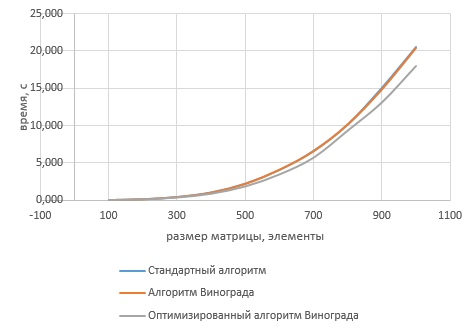
\includegraphics[scale=0.7]{t1.jpg}
        					\caption{\label{ris:test1}Замеры времени на матрицах с четным размером}
        				}
        			\end{figure}
        		
        			\begin{figure}[H]	
        				{
        					\centering
        					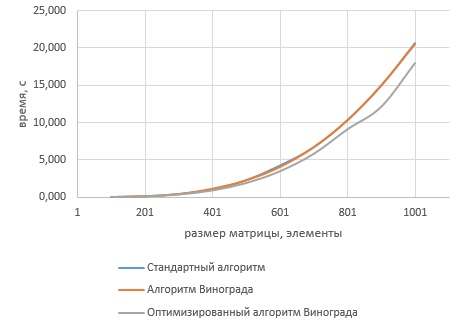
\includegraphics[scale=0.7]{t2.jpg}
        					\caption{\label{ris:test2}Замеры времени на матрицах с нечетным размером}
        				}
        			\end{figure}
	\end{center}

	Время работы алгоритма Винограда незначительно меньше стандартного алгоритма умножения, однако оптимизированная реализации имеет заметный прирост в скорости работы, на метрацах размером 1000х1000 уже около 18\%.

    \newpage

    \begin{center}
        \section*{Заключение}
        \addcontentsline{toc}{section}{Заключение}
    \end{center}
            \label{sec:ending}
        	\qquad В рамках лабораторной работы были рассмотрены и реализованы стандартный алгоритм умножения матриц и алгоритм Винограда. Была рассчитана их трудоемкость и произведены замеры времени работы реализованных алгоритмов. На основании этого произведено сравнение их эффективности. Оптимизированный алгоритм Винограда имеет заметный выйгрыш в эффективности работы по сравнению с остальными алгоритмами.
    \newpage

    \begin{center}        
        \begin{thebibliography}{}
        	\bibitem{litlink1}  Березкина Э. И. Математика древнего Китая / Отв. ред. Б.А.Розенфельд. — М.: Наука, 1980. — С. 173-206. — 312 с.   
        	\bibitem{litlink2}  Даан-Дальмедико А., Пейффер Ж. Пути и лабиринты. Очерки по истории математики: Пер. с франц. — М.: Мир, 1986. — С. 397.       	
        	
        \end{thebibliography}
    \end{center}

\end{document}
